% !TeX root = ../FoodSpy.tex
% \section{Aplicații web - noțiuni teoretice}

\section{Arhitectura client-server}
Arhitectura client-server se referă la configurația de calculatoare în care server-ul găzduiește și administrează resursele și serviciile folositoare clientului. Mai multe calculatoare sunt legate la un server central printr-o rețea sau conexiune la internet pentru a putea partaja resursele de calcul.\\ \\
Clientul solicită o resursă de pe server printr-o conexiune la rețea, solicitarea fiind prelucrată și livrată înapoi clientului de către server. În această arhitectură, clientul este consumatorul, acesta utilizează serviciile oferite de server, și deci server-ul este producătorul. Serviciile oferite de către server sunt: stocarea datelor, partajarea datelor, accesul la aplicații sau accesul direct către resursele de calcul ale server-ului.\\ \\
Clientul execută următoarele operații: trimite solicitări către server, așteaptă și primește răspuns de la server și este activ, în sensul că este cel care inițiază operația de tranzacție între acesta și server.
\\ \\
Serverul este inițial pasiv, așteaptă o cerere de la client, verifică autorizarea, ascultă și este pregătit să răspundă solicitărilor clientului, iar când aceste solicitări sunt primite, le tratează, prelucrează și le trimite înapoi clientului sub forma unui răspuns.
\\ \\
Arhitectura client-server prezintă o serie de avantaje când vine vorba de persistența datelor:
\begin{itemize}
	\item avantajul centralizării tuturor datelor pe un singur server înseamnă că se pot simplifica operațiile de securizare ale datelor. De asemenea, operațiile de actualizare de date sau de software pot fi mai ușor de realizat
	\item avantajul de a fi accesibilă ușor, clientul putând să se conecteze la server de oriunde
	\item costurile comunicațiilor sunt reduse deoarece pe rețea circulă mai puține date pentru că o parte din operațiile executate de aplicație sunt efectuate la client
	\item configurarea serverului este mai ușoară fiindcă singura sarcina a server-ului este de a prelucra baza de date
\end{itemize}


\section{Hypertext Transfer Protocol}
HTTP este protocolul care permite accesarea de resurse, cum ar fi documente HTML. Reprezintă piatra de temelie pentru orice schimb de date pe web și este un protocol client-server. Browser-ul web este clientul și trimite cereri către server. Un document HTML complet este reconstituit din rezultatul mai multor sub-documente primite ca răspuns de la server. Sub-documentele pot fi bucățile de text care compun conținutul paginii, descrierea structurii paginii, imagini sau script-uri.
\\ \\
Clienții și server-ele comunică printr-un schimb de mesaje individuale și nu printr-un flux de date. Mesajele trimise de către client se numesc cereri (din engl. ”requests”), iar mesajele primite înapoi din partea server-ului se numesc răspunsuri (din engl. ”responses”).

\begin{figure}[!htb]
	\centering
	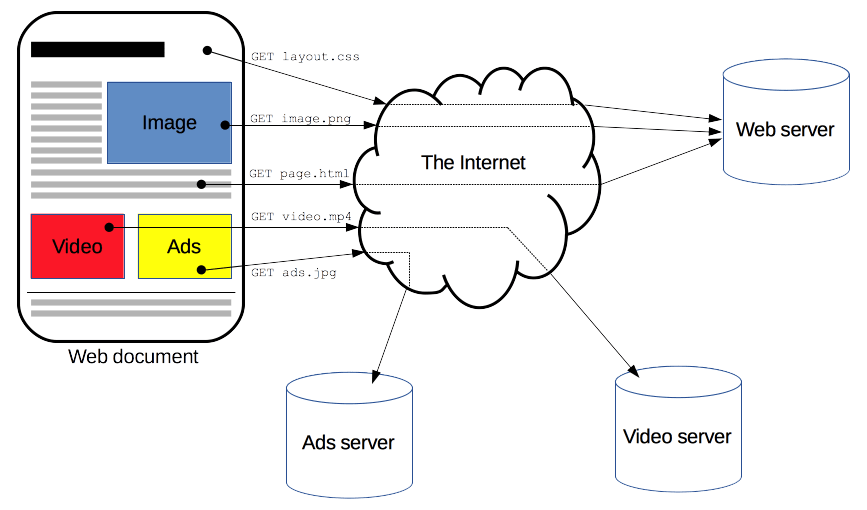
\includegraphics[width=1\textwidth]
	{../LaTeX/Images/http_fetch.PNG}
	\caption{Schimbul de mesaje între client și un server web}
	\label{fig:21}
\end{figure}

\subsection{Componentele unui sistem HTTP}
HTTP este un un protocol client-server, adică există o entitate care trimite cereri. Această entitate se numește ”user-agent” și este reprezentată de cele mai multe ori de un browser web, dar poate fi reprezentat și de un robot care menține un index pentru un motor de căutare.
\\ \\
Fiecare cerere se procesează în mod individual și întoarce un răspuns. Între browser și serverul care administrează cererile există nivelul de rețea și nivelul de transfer de date, format din router-e, modem-uri și altele. HTTP este deasupra acestor două nivele, deoarece face parte din nivelul de aplicație.
\\ \\
Pentru a afișa o pagină web, clientul trimite prima oară o cerere pentru aducerea documentului HTML care reprezintă pagina. Apoi, interpretează (din engl. ”parses”) documentul HTML și execută alte cereri. Aceste cereri corespund cu identificarea în fișier a script-urilor, opțiunilor de stilizare ale paginii (CSS) sau resursele media necesare, imagini și clipuri video. După ce toate aceste cereri au fost satisfăcute, browser-ul web pune toate părțile componente laolaltă și afișează pagina completă în fereastră.
\\ \\
O pagină web este un document ”hypertext”, adică poate conține legături către alte pagini web, accesibile la evenimentul de click al mouse-ului pe bucățile din text care reprezintă link-uri. Asta permite utilizatorilor să direcționeze clientul de pe o pagină pe alta și să navigheze pe web. Browser-ul este cel care interpretează aceste direcționări sub forma unor cereri HTTP de la care așteaptă răspuns. Răspunsul îl afișează utilizatorului sub forma unui mesaj clar.
\\ \\
La partea opusă a clientului stă server-ul, care așteaptă și administrează cererile primite. Un server nu este reprezentat neapărat de către o singură resursă de calcul. Folosind anumite soluții software, server-ul poate chiar partaja aceeași adresă IP cu alte server-e, folosind versiunea 1.1 a protocolului HTTP și antetul ”Host”. Antetul ”Host” specifică port-ul și gazda către care se trimite o cerere pentru a fi îndeplinită.

\subsection{Aspectele protocolului HTTP}
HTTP este gândit să fie simplu, extensibil și ”stateless”. ”Stateless” înseamnă că nu există o legătură între două cereri succesive, efectuate pe aceeași conexiune. Acest lucru ridică anumite probleme, deoarece un utilizator nu poate în mod coerent să interacționeze cu anumite pagini web, de exemplu, cu paginile web ale unui magazin online. Deși nucleul HTTP este ”stateless”, folosind cookie-uri HTTP se pot iniția așa numitele sesiuni ”stateful”. Folosind antetul unei cereri HTTP, cookie-urile se pot adăuga în antet, astfel încăt să permită creearea de sesiuni care partajează același context sau aceeași stare.

\subsection{Fluxul HTTP}
Se deschide o conexiune folosită pentru transportul cererii și al răspunsului.
Se trimite un mesaj HTTP, o cerere, după cum se poate observa în (Fig. \ref{fig:22}).

\begin{figure}[!htb]
	\centering
	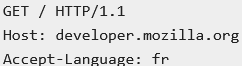
\includegraphics[width=0.5\textwidth]
	{../LaTeX/Images/http_message.PNG}
	\caption{Exemplu de mesaj HTTP}
	\label{fig:22}
\end{figure}

Răspunsul este ilustrat în (Fig. \ref{fig:23}). Acesta este citit de către client și interpretat.

\begin{figure}[!htb]
	\centering
	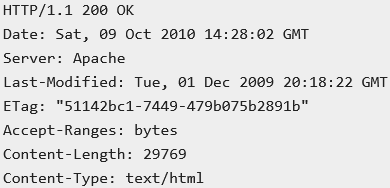
\includegraphics[width=0.8\textwidth]
	{../LaTeX/Images/http_response.PNG}
	\caption{Exemplu de răspuns HTTP}
	\label{fig:23}
\end{figure}

Pasul final este închiderea sau refolosirea conexiunii pentru alte cereri.

\subsection{Mesajele HTTP}
Există două tipuri de mesaje HTTP: ”request” și ”response”.
\\ \\
Un ”request” este compus din:
\begin{itemize}
  \item o metodă HTTP, de regulă ”GET” sau ”POST” care definește operația pe care clientul dorește să o efectueze
  \item calea către resursa de pe server dorită de client
  \item versiunea protocolului HTTP folosit
  \item anumite anteturi care oferă server-ului informații adiționale
  \item ”body”, dacă este vorba, de exemplu, de metoda ”POST” - acest ”body” poate conține o resursă trimisă de către client
\end{itemize}

Un exemplu de ”request” este ilustrat în (Fig. \ref{fig:24}).

\begin{figure}[!htb]
	\centering
	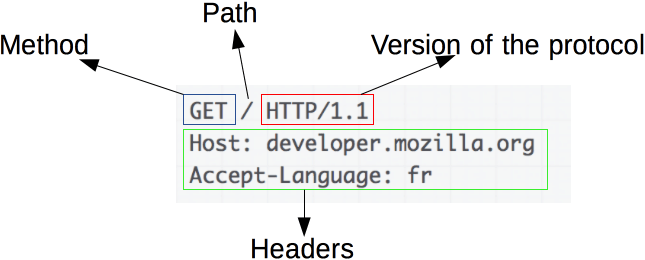
\includegraphics[width=0.7\textwidth]
	{../LaTeX/Images/http_request.PNG}
	\caption{Exemplu de ”request” HTTP}
	\label{fig:24}
\end{figure}

Un ”response” este compus din:
\begin{itemize}
  \item ”status code” care indică faptul că cererea a fost îndeplinită sau nu
  \item ”status message” care descrie pe scurt ”status code”
  \item versiunea protocolului HTTP
  \item anteturi
  \item ”body”
\end{itemize}

Un exemplu de ”response” este ilustrat în (Fig. \ref{fig:25}).

\begin{figure}[!htb]
	\centering
	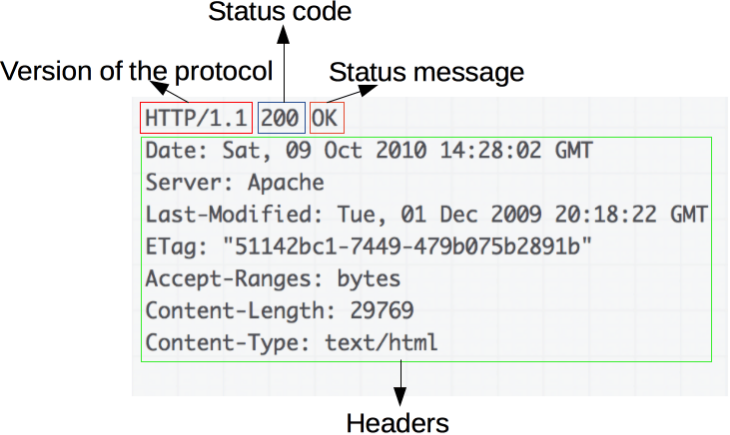
\includegraphics[width=0.7\textwidth]
	{../LaTeX/Images/http_response-ex.PNG}
	\caption{Exemplu de ”response” HTTP}
	\label{fig:25}
\end{figure}


\section{Aplicație web vs. site web}
Deși se accesează în același fel și arată la fel, o aplicație web nu este un website.\\
O aplicație web este construită cu scopul de a interacționa cu utilizatorul, în timp ce un website doar servește conținut static, conținut care nu poate fi afectat de către vizitator.
\\ \\
Website-ul este structurat pe mai multe pagini care au adrese web diferite și care indică resurse web diferite, în timp ce, de regulă, o aplicație web ”rescrie” în mod dinamic pagina curentă pe care se află utilizatorul; această ”rescriere” stă la baza așa numitelor ”single-page application”.
\\ \\
Pentru a putea interacționa cu aplicația web, un utilizator trebuie autentificat și autorizat \footnote{Dacă luăm un exemplu cu un club, prin autentificare se înțelege procesul de identificare a vârstei unui petrecăreț, pe baza unui buletin, în vreme ce prin autorizare se înțelege acordarea unor privilegii speciale acestui petrecăreț, accesul în zona VIP, în zona DJ-ului, și așa mai departe.}, în vreme ce vizitatorul unui website poate cel mult să se înscrie pe o listă de corespondență de unde poate primi notificări din partea administratorul website-ului.
\\ \\
Un website este un mod de afișare structurată a informației. Este un produs complet, accesibil printr-un browser web, nu necesită compilare, doar actualizarea structurii și informației, acolo unde este cazul, fără nevoia de implementare (din engl. ”deployment”).
\\ \\
O aplicație web este o soluție software sau un program, accesibil printr-un browser web. Spre deosebire de programele desktop, aplicația web este valabilă pe orice platformă deoarece sistemele de operare desktop suportă majoritatea browser-elor web moderne. De asemenea, pe sistemele de operare mobile nu este necesară aprobarea într-un magazin de aplicații (App Store sau Google Play) pentru a fi folosite pe aceste dispozitive. Aplicațiile web sunt mai ușor de întreținut deoarece folosesc același cod-sursă pentru toate platformele și mai mult decât atât, nu este necesară actualizarea lor de către utilizatori, cum este cazul aplicațiilor mobile.
\\ \\
Aplicația web are avantajul scalabilității și găzduirii în cloud. Poate fi folosită pe orice platformă, este modulară și suportă testarea acesteia folosind teste automate.


\section{REST API}
Acronimul REST vine de la ”representational state transfer” și este un stil arhitectural menit pentru construirea de aplicații web scalabile.
O interfață de programare (din engl. ”API”) REST are caracter ”RESTful” dacă se conformează constrângerilor impuse de stilul arhitectural REST.
\\ \\
Pentru a implementa un asemenea API, există câteva cerințe care trebuie îndeplinite și anume:

\begin{itemize}
  \item implementarea unei arhitecturi client-server compusă din clienți, server-e și resurse și folosirea protocolului HTTP pentru administrarea cererilor și răspunsurilor. Clientul trimite o cerere pe care server-ul o poate respinge sau o poate îndeplini prin oferirea unui răspuns adecvat.
  \item comunicare ”stateless” între client și server, astfel încât nicio informație de la client nu este stocată între mai multe cereri succesive, iar cererile sunt tratate în mod individual, separat și neconectat. Clientul și server-ul sunt prinși într-o secvență cerere-răspuns, în care clientul inițiază o cerere, iar server-ul răspunde. La cererile ulterioare, server-ul nu cunoaște răspunsurile pe care l-a oferit anterior.
  \item posibilitatea stocării în cache pentru facilitarea comunicării dintre client și server. Cererile inițiate de client au caracter independent. La momentul repetării uneia dintre aceste cereri, răspunsul este stocat în cache la nivelul clientului. Când clientul repetă o cerere, aceasta nu mai ajunge până la server, ci este oferit răspunsul direct din cache.
  \item folosirea unei interfețe uniforme între componentele arhitecturii astfel încât informația poate fi transferată sub o formă standard:
	\begin{itemize}
		\item resursele cerute de client sunt identificabile și separate de reprezentările oferite înapoi clientului
		\item resursele pot fi manipulate de către client via reprezentările oferite, deoarece acestea conțin suficiente informații astfel încât să permită manipularea lor
		\item mesajele oferite alături de răspunsul de la server trebuie să fie ușor de interpretat, astfel încât clientul să le poată procesa
	\end{itemize}
  \item un sistem stratificat care organizează fiecare tip de server responsabil pentru îndeplinirea cererilor, în ierarhii, invizibile clientului. Asta face posibilă implementarea unui strat adițional, numit ”middleware” care stă între client și server. Clientul poate interacționa cu stratul ”middleware”, dar clientul nu trebuie să recunoască prezența acestuia.
  \item opțional, se poate implementa ”code-on-demand”, prin care se permite trimiterea codului executabil de la server către client, la cerere, extinzând astfel funcționalitatea API-ului
\end{itemize}

REST este un set de constrângeri arhitecturale, nu un protocol sau un standard. Dezvoltatorii de interfețe de programare ”RESTful” pot deci să implementeze acest stil arhitectural în mai multe feluri, dar respectând cerințele.
\\ \\
REST constituie o cale de acces către resursele care sunt stocate într-un anume mediu. De exemplu, un server poate stoca o colecție de documente și imagini, iar fiecare document și fiecare imagine reprezintă o astfel de resursă. REST definește un serviciu care spune cum ar trebui să fie implementat accesul către aceste resurse.
\\ \\
Definiție pentru o resursă web. O aplicație web poate fi folosită, de exemplu, pentru accesul la datele despre angajații unei firme. Fiecărui angajat îi corespunde o înregistrare în baza de date. Dacă URL-ul pentru aplicația web este ”http://demo.a3drian.com”, la datele despre unul dintre angajați se ajunge printr-o cerere către URL-ul\\”http://demo.a3drian.com/employee/1”. La momentul îndeplinirii acestei cereri, se aduc datele despre angajatul care are ”ID”-ul ”1”.
\\ \\
Definiție pentru metodele HTTP. Aceste metode descriu felul în care clientul dorește să interacționeze cu o resursă. Principalele metode sunt:
\begin{itemize}
  \item GET
  \item POST
  \item DELETE
  \item PUT
  \item PATCH
\end{itemize}

Metodele sunt explicate în detaliu în (Tabelul \ref{fig:26}).

\begin{table}[]
\centering
\resizebox{\textwidth}{!}{%
\begin{tabular}{lll}
URL          & metodă & funcționalitate                                                             \\
\hline
employees/10 & GET    & aduce datele despre un singur angajat (o singură resursă)                   \\
employees    & GET    & întoarce întreaga listă de angajați (toate resursele)                       \\
employees    & POST   & creează o nouă resursă cu datele primite în corpul (”body”) cererii         \\
employees/10 & DELETE & șterge resursa cu ID-ul ”10”                                                \\
employees/10 & PUT    & înlocuiește conținutul unei resurse cu datele primite în cerere             \\
employees/10 & PATCH  & înlocuiește doar o parte a conținutului unei resurse cu datele primite în cerere
\end{tabular}%
}
\caption{Descrierea în detaliu a metodelor HTTP}
\label{fig:26}
\end{table}

Definiție pentru anteturi. Anteturile sunt folosite pentru a trimite server-ului informații adiționale legate de cerere. Spre exemplu, ”Content-Type: text/html; charset=UTF-8” este antetul care impune server-ului să răspundă cu o resursă în format ”text/html” și având setul de caractere ”UTF-8”. Un alt exemplu este ”Authorization” - antetul care conține credențialele necesare clientului pentru procesul de autentificare.
\\ \\
Definiție pentru ”body”-ul cererii. O cerere poate să conțină informații sub formă de date. De regulă, datele sunt trimise împreună cu o cerere atunci când se execută metoda ”POST”. Metoda ”POST” comunică server-ului faptul că dorește să adauge o nouă resursă. Astfel, în corpul (”body”) cererii sunt conținute datele pe care server-ul le folosește pentru adăugarea resursei noi.
\\ \\
Definiție pentru ”body”-ul răspunsului. Acesta reprezintă corpul principal al răspunsului. Referindu-ne la exemplul de mai sus, când URL-ul pentru aplicația web era ”http://demo.a3drian.com”, atunci când se face o cerere ”GET” la URL-ul\\”http://demo.a3drian.com/employee/1” server-ul poate întoarce datele despre angajatul cu ”ID”-ul ”1” sub formă de JSON sau sub formă de XML.
\\ \\
Definiție pentru ”status code”. Reprezintă o colecție de numere întregi și constituie codurile care se returnează alături de răspunsul venit de la server. ”200” este codul care se atașează răspunsului, atunci când cererea clientului a fost îndeplinită cu succes. ”404” este folosit în momentul în care resursa cerută de client nu a fost găsită pe server, iar ”504” este codul rezultat atunci când server-ul este offline. Alături de aceste coduri, server-ul trimite și un scurt mesaj. Lângă ”200” se atașează ”OK”, lângă ”404” server-ul întoarce mesajul ”Not found”, iar lângă ”504” mesajul returnat este ”Gateway timeout”.